\documentclass[12pt, Letterpaper]{article}

\usepackage[utf8]{inputenc}
\usepackage{amssymb}
\usepackage{graphicx}
\graphicspath{{img}}

\begin{document}
\begin{center}
\Huge\textbf{Informe Prácticas de Programación Primer Año}
\vspace{0.5em}\\
\large{David Michel García Batista}\\
\small{Julio de 2023}
        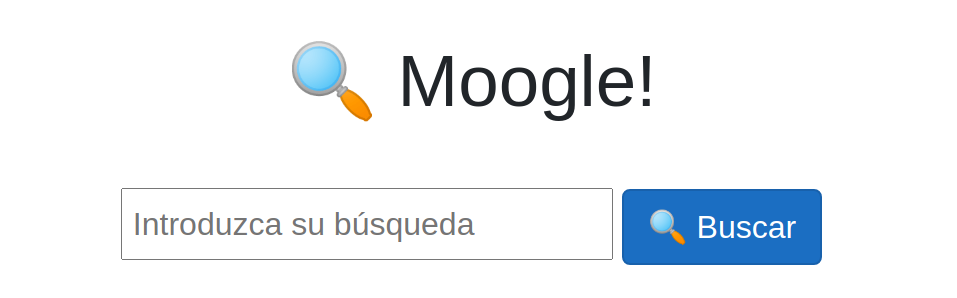
\includegraphics[width=13cm]{moogle-1.png}
        \end{center}
\begin{abstract}
    \textbf{\textit{¿En que consiste este proyecto? ¿Qué es Moogle!}}\\
Moogle! es una aplicación web (cuyo nombre desborda originalidad) que constituye un modelo de búsqueda vectorial con
la finalidad de encontrar en un conjunto de documentos aquellos más relevantes y relacionados con la información
deseada. Ésta información será un conjunto de palabras introducidas por el usuario en lo que
denominaremos \underline{Query}.
\end{abstract}

\newpage
Para poder llevar a cabo dicha tarea es necesario de alguna manera precisar o mejor dicho, cuantificar que tan 
relevante es cada documento con respecto a esta Query ingresada para luego poder compararlos y determinar aquellos
mas importantes. Pues para esto utilizaremos dos procesos fundamentales, el TF-IDF (Term Frequency-Inverse Document 
Frequency) y la similitud de cosenos. Ahora procedemos a describir como funciona esto.\\

Lo primero es comprender en que consiste el TF-IDF y la similitud de cosenos:
\begin{itemize}
    \item \textbf{\underline{TF}}: No es más que la frequencia con la que aparece una palabra en un texto dependiendo
     de la cantidad de veces que aparece (Si una palabra aparece 5 veces en un texto de 100 palabras su TF=0,05)\\
        Fórmula: \[TF=\frac{t}{td} \]
        Donde:
        \begin{itemize}
        \item \textbf{t} representa la cantidad de apariciones del término en el documento. 
        \item \textbf{td} la cantidad de términos que tiene el documento.
        \end{itemize} 
        \item \textbf{\underline{IDF}}: Su función es básicamente determinar la rareza de una palabra, o sea, 
        analiza la aparición de una palabra en todos los textos por lo que mientras más común sea un término mas baja
        será su puntuación, de esta manera se logra despreciar aquellas palabras que se repiten mucho como las 
        preposiciones, dándole prioridad a aquellas palabras "raras" que aparecen pocas veces y se sobrentiende que 
        sean más importantes.
        
        Fórmula: \[IDF=\log (\frac{N}{DF}) \] 
        Donde:
        \begin{itemize}
            \item \textbf{N} representa el número total de documentos en la colección.
            \item \textbf{DF} es el número de documentos en los que aparece un término específico.
        \end{itemize}
          
        \item \textbf{\underline{Similitud de coseno}}: Es un concepto medianamente abstracto, pues permite analizar 
        vectores en el espacio mediante una formúla para determinar el ángulo entre ellos, mientras más pequeño sea el
        ángulo más cercano estará el valor de su coseno a 1 y por ende mayor similitud tendrá. Ésto es lo que usaremos
        para comparar cada documento con la Query y así determinar la relevancia.
        Fórmula: \[sim(A,B)=cos(\theta )=\frac{A\bigodot B}{\| A \| * \| B \|} \] 
        Donde:
        \begin{itemize}
            \item \textbf{A} y \textbf{B} son dos \underline{vectores}.
            \item $(A\bigodot B)$ representa el producto escalar entre los vectores A y B, es el producto de los  
            valores correspondientes de los componentes sumados entre sí.
            \item $\| A \|$ y $\| B\|$ representan las normas de los vectores A y B. La norma de un vector es la 
            magnitud o longitud del vector y se calcula como la raíz cuadrada de la suma de los cuadrados de sus 
            componentes.\\

            En la siguiente figura se ve una representación gráfica de esta similitud de coseno para una mejor comprensión
            \begin{center}
            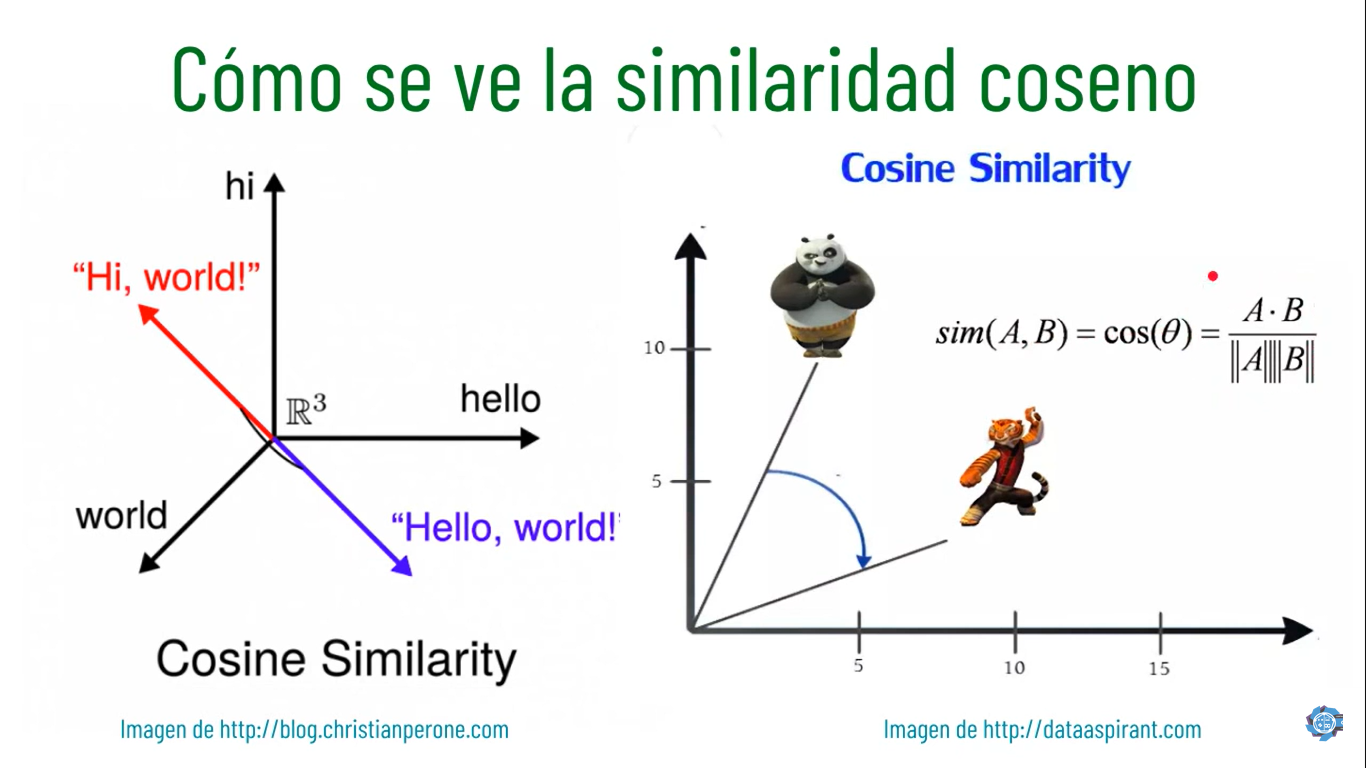
\includegraphics[width=11cm $$  $$]{Sim Cos.png}
            \end{center}
        \end{itemize}
    \end{itemize}
    \newpage
    El principio del funcionamiento del proyecto se encuentra dentro de \textbf{Moogle Engine} el cual contiene las 
    distintas clases que realizarán las funciones y procesos del programa. La idea es procesar la información de cada
    documento que se encuentre dentro de la carpeta Content y crear un diccionario para cada documento que contenga
    una relacion de cada palabra del texto y su correspondiente \textbf{TF-IDF}, luego construir una Base de Datos 
    que contenga a todos los documentos y sus relevancias con respecto a la \textbf{Query}. Ahora, para determinar el
    valor de dicha relevancia será necesario procesar la Query de la misma manera que un documento para calcular su
    TF-IDF, una vez logrado ésto podremos aplicar la fórmula de la similitud de cosenos para calcular estos valores y
    luego compararlos para dar como resultado de la búsqueda aquellos con mayor relevancia. Como no sería eficiente 
    imprimir todo el documento como resultado, lo mejor es asignarle el título y un fragmento del texto llamado 
    \textbf{Snippet} que estará relacionado con la Query para ser imprimidos en pantalla.
    
    Todo este funcionamiento estará respaldado por varias clases que ejecutarán sus funciones.\\
    \begin{itemize}
        \item \textbf{Clase Document} Procesa la información de los documentos individualmente utilizando:
        \begin{itemize}
            \item Directory.GetCurrentDirectory: Obtener las localizaciones de los archivos .txt
            \item Directory.GetFiles: Para conseguir el contenido de dichos archivos.
            \item Método Split Text: Para separar los textos por palabas y llevarlas a minúscula usando.ToLower.
            \item Método Get Title: Para conseguir el título de los txt.
            Támbién esta clase servirá para construir el diccionario con la relación palabra y TF-IDF de cada documento.
        \end{itemize}
        \item \textbf{Clase TF-IDF} Estará encaminada específicamente al cálculo de este parámetro. 
        \item \textbf{Clase Database} Siguiendo la línea de originalidad en los nombres será la encargada de 
        construir la base de datos con la información de todos los documentos y la Query para poder aplicar la 
        similitud de cosenos y determinar las relevancias, finalmente teniendo todo lo necesario para dar los 
        resultados de la búsqueda.
    \end{itemize} 
\end{document}